\documentclass[10pt,pdf,hyperref={unicode}]{beamer}

% \documentclass[aspectratio=43]{beamer}
% \documentclass[aspectratio=1610]{beamer}
% \documentclass[aspectratio=169]{beamer}

\usepackage{lmodern}
\usepackage[russian]{babel}

% подключаем кириллицу 
%\usepackage[T2A]{fontenc}
\usepackage[T1]{fontenc}
\usepackage[utf8]{inputenc}
\usepackage{bm}

% отключить клавиши навигации
\setbeamertemplate{navigation symbols}{}

% тема оформления
\usetheme{Madrid}

% цветовая схема
\usecolortheme{whale}

\title[UDE]{Универсальные дифференциальные уравнения}   
\subtitle{Комбинация лучших сторон разных подходов.}
\author{Влад Темкин} 



\institute[HSE] % (optional)
{
	Высшая Школа Экономики\\
	Факультет Физики
}

\date[\today]
{Стохастические процессы и моделирование}

\AtBeginSection[]
{
	\begin{frame}
		\frametitle{План доклада}
		\framesubtitle{Основные моменты}
		\tableofcontents[currentsection]
	\end{frame}
}

\begin{document}
	
	\begin{frame}
		\titlepage
	\end{frame} 
	
	
	\begin{frame}
		\frametitle{План доклада} 
		\framesubtitle{Основные моменты}
		\tableofcontents[pausesections]
	\end{frame}


	\section{Подходы к описанию мира}
	
		\subsection{Физические модели}
		
			\begin{frame}
				\frametitle{Подходы к описанию мира} 
				\framesubtitle{Физические модели}
					\begin{columns}
						\column{0.5\linewidth}
						\begin{center}
							\begin{itemize}
								\item<2-> хорошо интерполируют (очень хорошо)
								\item<3-> легко интерпретировать 
								\item<4-> указывают на структуру процесса
								\item<5-> нужно понимать хоть что-то о мире
								\item<6-> проигрывают другим моделям (а именно машинному обучению), когда речь идёт о предсказаниях просто из набора данных
							\end{itemize}
						\end{center}
						\column{0.5\linewidth}
							\begin{displaymath}
								\frac{d}{dt}\frac{\partial \mathcal{L}}{\partial \dot{x}} - \frac{\partial \mathcal{L}}{\partial x} = 0
							\end{displaymath}
							\newline
							\begin{displaymath}
								\left\{\begin{gathered}
									\nabla \cdot \vec{D} = 4\pi	\rho\\
									\nabla \cdot \vec{B} = 0 \\
									\nabla \times \vec{E} = \frac{1}{c}\frac{\partial \vec{B}}{\partial t} \\
									\nabla \times \vec{H} = \frac{4\pi}{c}\vec{j} + \frac{1}{c}\frac{\partial \vec{D}}{\partial t}
								\end{gathered}\right.
							\end{displaymath}
							\newline
							\begin{displaymath}
								u' = f(u,p,t)
							\end{displaymath}
					\end{columns}
			\end{frame}
		
		
		\subsection{Машинное обучение}
		
			\begin{frame}
				\frametitle{Подходы к описанию мира} 
				\framesubtitle{Машинное обучение}
					\begin{columns}
						\column{0.5\linewidth}
							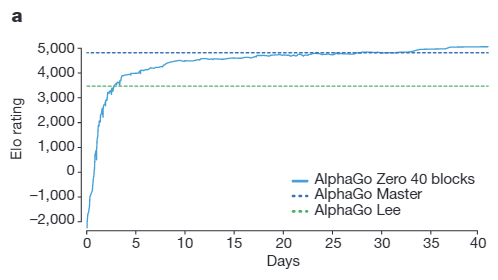
\includegraphics[width=\linewidth]{alphago.png}
							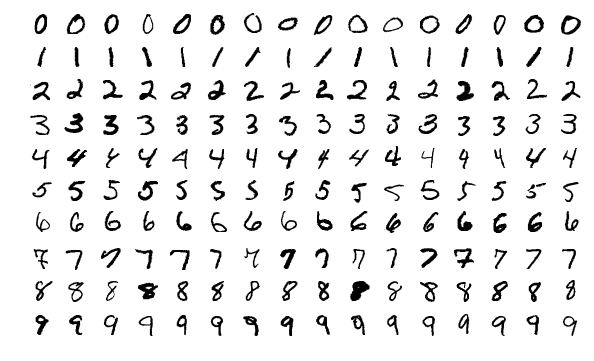
\includegraphics[width=\linewidth]{mnist.png}
						\column{0.5\linewidth}
						\begin{center}
							\begin{itemize}
								\item<2-> может решить почти любую ограниченную задачу
								\item<3-> превосходит человека во многих областях
								\item<4-> потенциал кажется безграничным (обучение с подкреплением)
								\item<5-> сложно интерпретировать
								\item<6-> не всегда хорошо интерполирует  
								\item<7-> требуется много данных
							\end{itemize}
						\end{center}
					\end{columns}
			\end{frame}
			
			
	\section{Комбинирование двух подходов}
		
		\begin{frame}
			\frametitle{Комбинирование двух подходов} 
			\framesubtitle{Различные практики}
				\begin{block}{Универсальная теорема аппроксимации}
					Нейронная сеть может аппроксимировать любую непрерывную функцию $R^n \to R^m$ с любой заданной точностью.
				\end{block}  
				\begin{itemize}
					\item<2-> Physical Informed Neural Networks (PINNs):
					\begin{displaymath}
					\begin{gathered}
						u_t + \mathcal{N}[u,\lambda] = 0\\
						f = u_t + \mathcal{N}[u,\lambda], u = NN
					\end{gathered}
					\end{displaymath}
					\item<3-> Нейронные обыкновенные дифференциальные уравнения (NODE) (и не только обыкновенные):
					\begin{displaymath}
						u' = NN(u)
					\end{displaymath}
					\item<4-> Универсальные дифференциальные уравнения
				\end{itemize}
		\end{frame}
	
		\begin{frame}
			\frametitle{Комбинирование двух подходов} 
			\framesubtitle{Пример вшитой природы}
			\begin{center}
				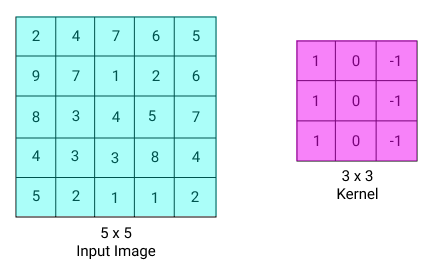
\includegraphics[width=0.45\linewidth]{cnn.png}
			\end{center}
				\begin{columns}
					\column{0.6\linewidth}
					\begin{displaymath}
						\begin{gathered}
							\Delta u = u_{xx} + u_{yy} = \\
							= \frac{u(x+\Delta x,y) - 2u(x,y) + u(x-\Delta x, 	y)}{\Delta x^2} + \\
							+\frac{u(x,y + \Delta y) - 2u(x,y) + u(x, y - \Delta y)}{\Delta y^2}
						\end{gathered}
					\end{displaymath}
					\column{0.4\linewidth}
					\begin{center}
						\begin{tabular}{ c c c }
							0 & 1 & 0 \\ 
							1 & -4 & 1 \\  
							0 & 1 & 0
						\end{tabular}
					\begin{displaymath}
						\begin{gathered}
							u_t = \Delta u \\
							u_t = CNN(u)
						\end{gathered}
					\end{displaymath}
					\end{center}
				\end{columns}
		\end{frame}
		
				
	\section{Универсальные дифференциальные уравнения}
	
		\begin{frame}
			\frametitle{Универсальные дифференциальные уравнения} 
			\framesubtitle{Что это?}
				\begin{center}
				 	WolframMathWorld: универсальные дифференциальные уравнения -- это такие дифференциальные уравнения, чьи решения могут приблизить любую непрерывную функцию с заданной точностью. 
				 	\begin{block}{Бриггс, 2002:}
				 		\begin{displaymath}
				 		y''''y'^2 - 3y'''y''y'+2(1-n^{-2})y''^3=0 \text{ для  } n > 3
				 		\end{displaymath}
				 	\end{block}
			 		\hfill\break
			 		\hfill\break
			 		\hfill\break
				 	 \pause
					Есть вариант попроще?
				 \end{center}
		\end{frame}
	
		\begin{frame}
			\frametitle{Универсальные дифференциальные уравнения} 
			\framesubtitle{Что это?}
			\begin{center}
				\begin{itemize}
					\item<1-> Пусть у нас есть какая-то информация об интересующей нас системе. Допустим, мы знаем, как эволюционировала бы какая-то её часть, если бы она существовала отдельно. Тогда можем написать дифференциальное уравнение, описывающее эту эволюцию:
					\begin{displaymath}
						u' = f(u, p, t),
					\end{displaymath}
					где $u$ -- какая-то наблюдаемая величина, $t$ -- время, $p$ -- прочие параметры системы. 
					\item<2-> А что, если эта часть окажется не изолирована? Наше дифференциальное уравнение, скорее всего, окажется уже неверным... 
					\item<3-> Что делать?
				\end{itemize}
			\end{center}
		\end{frame}
	
		\begin{frame}
			\frametitle{Универсальные дифференциальные уравнения} 
			\framesubtitle{Что это?}
			\begin{center}
				\begin{itemize}
					\item<1-> Добавим в правую часть дополнительное слагаемое, не уточняя его природу:
					\begin{displaymath}
						u' = f(u, p, t) + U_\theta(u),
					\end{displaymath}
					где $U_\theta$ -- универсальный аппроксиматор, то есть любая непрерывная функция.
					\item<2-> Все новые эффекты оказываются учтены в $U_\theta$!
					\item<3-> Но где взять информацию о нём?..
					\item<4-> Обучить нейронную сеть по собранным о системе данным!
				\end{itemize}
			\end{center}
		\end{frame}
	
		\begin{frame}
			\frametitle{Универсальные дифференциальные уравнения} 
			\framesubtitle{Что это?}
			\begin{block}{Рецепт 1}
				Универсальное дифференциальное уравнение $=$ известное уравнение $+$ аппроксимированные неизвестные слагаемые
			\end{block}
			\pause
			\begin{block}{Рецепт 2}
				Аппроксимация неизвестных слагаемых $=$ данные о системе $+$ машинное обучение
			\end{block}
		
		\end{frame}
	
		\begin{frame}
			\frametitle{Универсальные дифференциальные уравнения} 
			\framesubtitle{Алгоритм действий}
					\begin{enumerate}
						\item<2-> Определить известные части модели. Построить по ним UODE.
						\item<3-> Обучить нейронную сеть (или любой другой универсальный аппроксиматор), чтобы найти неизвестные механизмы.
						\item<4-> С помощью SINDy свести неизвестные части к механистическим слагаемым.
						\item<5-> Проверить то, что полученные законы правдоподобны.
						\item<6-> Экстраполировать полученную модель, исследовать предельные случаи.
						\item<7-> Получить новые данные и проверить на них полученную модель.
					\end{enumerate}
		\end{frame}
	
	
	\section{Вспомогательные инструменты}
	
		\subsection{алгортим SINDy}
		
			\begin{frame}
				\frametitle{Вспомогательные инструменты} 
				\framesubtitle{Алгоритм SINDy}
				\begin{columns}
					\column{0.35\linewidth}
					\begin{itemize}
						\item<1-> Sparse
						\item<1-> Identification of
						\item<1-> Nonlinear
						\item<1-> Dynamics
					\end{itemize}
					\column{0.65\linewidth}
					\begin{itemize}
						\item<2-> Собрать данные: "координаты" и их "производные"
						\item<2-> Составить библиотеку базисных функций
						\item<2-> Решить задачу регрессии
						\item<2-> Выбрать простейшее решение
					\end{itemize}
				\end{columns}
			\pause[3]
			\begin{center}
				\hfill\break
				\hfill\break
				\hfill\break
				\hfill\break
				Everything should be made as simple as possible, but no simpler.
			\end{center}
			\end{frame}
		
			\begin{frame}
				\frametitle{Вспомогательные инструменты} 
				\framesubtitle{Алгоритм SINDy}
				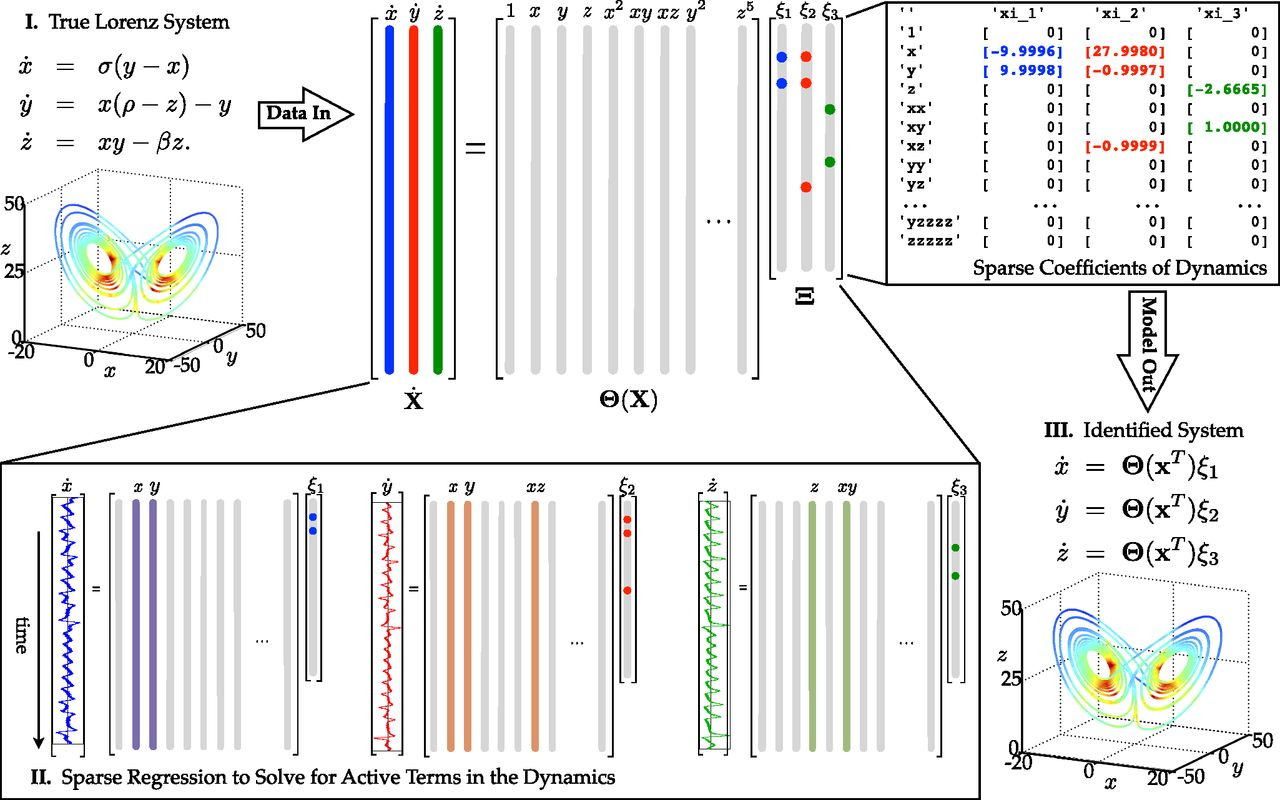
\includegraphics[width=\linewidth]{sindy.jpg}
			\end{frame}
		
		
	\section{Примеры применения UDE}
	
		\begin{frame}
			\frametitle{Примеры применения UDE} 
				\begin{itemize}
					\item Обыкновенные универсальные дифференциальные уравнения
					\begin{displaymath}
						u' = f(u,p,t) + U_\theta(u)
					\end{displaymath}
					\item Универсальные нейронные дифференциальные уравнения:
					\begin{displaymath}
						u_t = U_\theta(u) + D\cdot CNN(u)
					\end{displaymath}
					\item Многомерные универсальные дифференциальные уравнения в частных производных
					\item Универсальные алгебро-дифференциальные уравнения
					\item Стохастические универсальные дифференциальные уравнения
					\item Любые другие, где можно придумать, как заменить часть слагаемых на универсальный аппроксиматор.
				\end{itemize}  
		\end{frame}
	
		
		\subsection{Модифицированная модель SEIR}
		
			\begin{frame}
				\frametitle{Примеры применения UDE} 
				\framesubtitle{Модифицированная модель SEIR}
					\begin{center}
						\begin{displaymath}
							\begin{gathered}
							S' = -\beta_0 F \frac{S}{N} - \beta \frac{S I }{N} - \mu S \hfill susceptible\\
							E' = \beta_0 F \frac{S}{N} + \beta \frac{S I }{N} - (\sigma + \mu)E \hfill exposed \\
							I' = \sigma E - (\gamma + \mu) I \hfill infected\\
							R' = \gamma I - \mu R \hfill removed\\
							N' = -\mu N \hfill population\\
							D' = d\gamma I - \lambda D \hfill severe cases\\
							C' = \sigma E \hfill cumulative cases
							\end{gathered}
						\end{displaymath}
						\begin{displaymath}
							\beta = \beta_0 (1 - \alpha) (1 - \frac{D}{N})^\kappa
						\end{displaymath}
					\end{center}
			\end{frame}
		
			\begin{frame}
				\frametitle{Примеры применения UDE} 
				\framesubtitle{Модифицированная модель SEIR}
				\begin{center}
					\begin{figure}[h!]
						\begin{minipage}{.4\textwidth}
							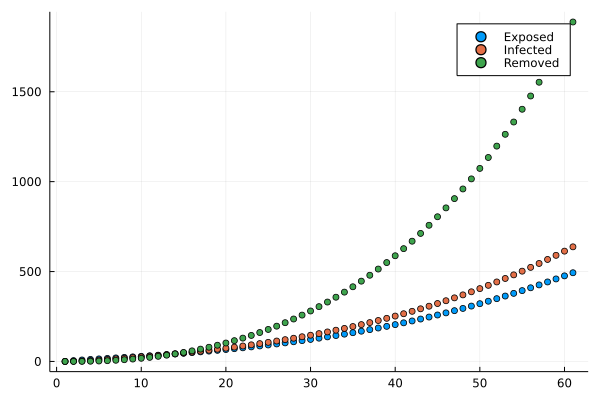
\includegraphics[width=\linewidth]{initial1.png}
							\caption{Решение исходной системы уравнений.}
							\centering
						\end{minipage}
						\begin{minipage}{.4\textwidth}
							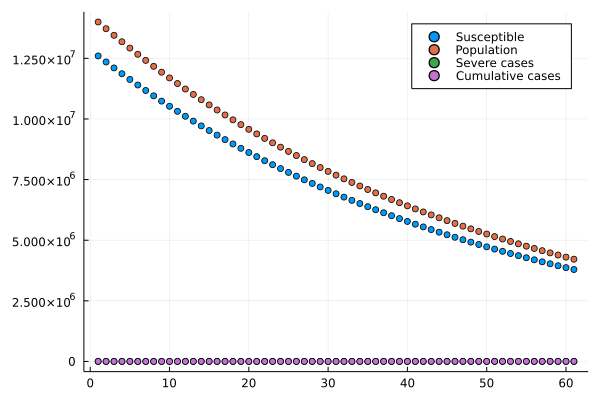
\includegraphics[width=\linewidth]{initial2.png}
							\caption{То же самое, другие величины.}
							\centering
						\end{minipage}
						\centering
					\end{figure}
				\end{center}
			\end{frame}
		
			\begin{frame}[fragile]
				\frametitle{Примеры применения UDE} 
				\framesubtitle{Модифицированная модель SEIR: Neural ODE}
					\begin{columns}
						\column{0.45\linewidth} 
						\begin{center}
							Определим NODE:
							\begin{displaymath}
							\frac{d}{dt}X = \mathcal{NN}(X)
							\end{displaymath}
						\end{center}
						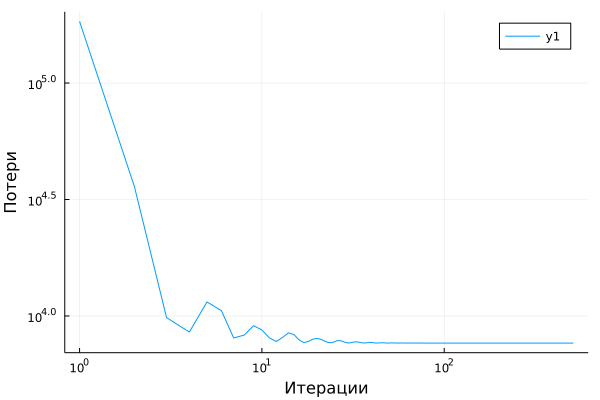
\includegraphics[width=.9\columnwidth]{neuralode_loss.png}
						\column{0.45\linewidth}
						\begin{verbatim}
							NN=FastChain(...)
							loss=sum(abs2,data.-solve(prob))
						\end{verbatim}
						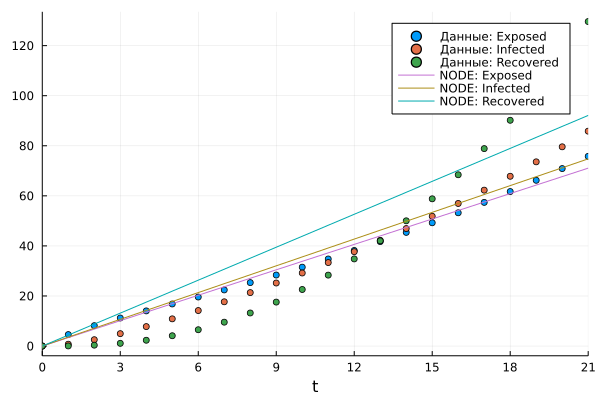
\includegraphics[width=.9\columnwidth]{neuralode_train.png}
					\end{columns}
			\end{frame}
		
			\begin{frame}
				\frametitle{Примеры применения UDE} 
				\framesubtitle{Модифицированная модель SEIR: Neural ODE}
				\begin{center}
					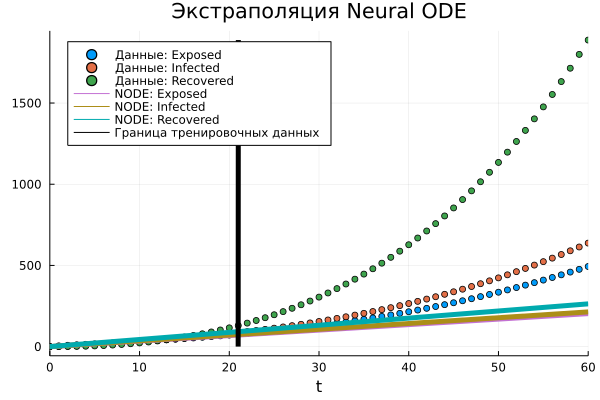
\includegraphics[width=0.8\linewidth]{neuralode_extrapolation.png}
				\end{center}
			\end{frame}
			
			
			\begin{frame}
				\frametitle{Примеры применения UDE} 
				\framesubtitle{Модифицированная модель SEIR}
				\begin{center}
					\begin{displaymath}
					\begin{gathered}
					S' = -\beta_0 F \frac{S}{N} - \mathcal{NN} - \mu S \\
					E' = \beta_0 F \frac{S}{N} + \mathcal{NN} - (\sigma + \mu)E\\
					I' = \sigma E - (\gamma + \mu) I\\
					R' = \gamma I - \mu R\\
					N' = -\mu N\\
					D' = d\gamma I - \lambda D\\
					C' = \sigma E
					\end{gathered}
					\end{displaymath}
				\end{center}
			\end{frame}
		
		
			\begin{frame}
				\frametitle{Примеры применения UDE} 
				\framesubtitle{Модифицированная модель SEIR}
				\begin{center}
					\begin{figure}[h!]
						\begin{minipage}{.45\textwidth}
							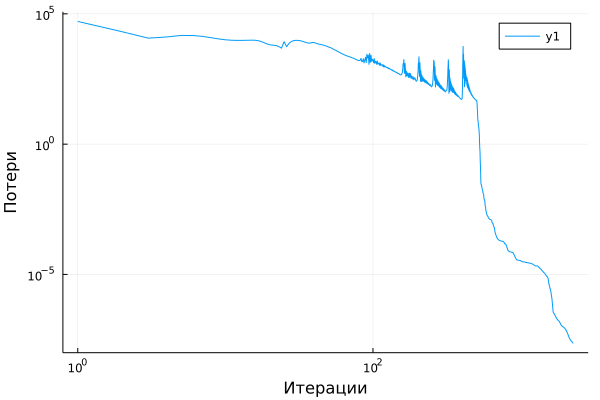
\includegraphics[width=\linewidth]{uode_loss.png}
							\caption{Функция потерь при обучении UODE.}
							\centering
						\end{minipage}
						\begin{minipage}{.45\textwidth}
							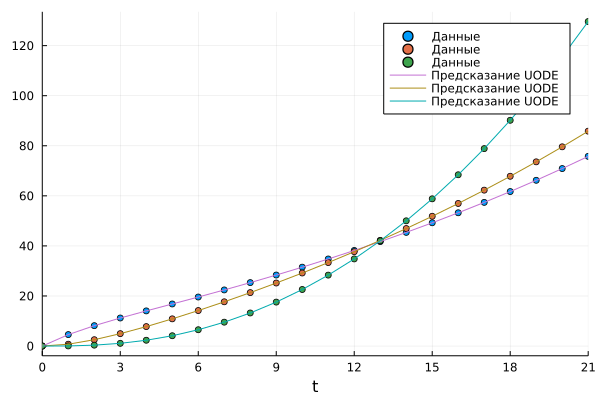
\includegraphics[width=\linewidth]{uode_prediction_train.png}
							\caption{Обучающая выборка.}
							\centering
						\end{minipage}
						\centering
					\end{figure}
				\end{center}
			\end{frame}
		
			\begin{frame}
				\frametitle{Примеры применения UDE} 
				\framesubtitle{Модифицированная модель SEIR}
				\begin{center}
					\begin{figure}[h!]
						\begin{minipage}{.45\textwidth}
							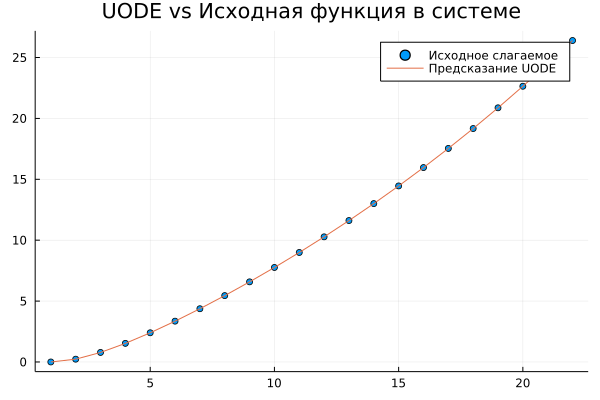
\includegraphics[width=\linewidth]{uode_estimated_exposure.png}
							\caption{Функция потерь при обучении UODE.}
							\centering
						\end{minipage}
						\begin{minipage}{.45\textwidth}
							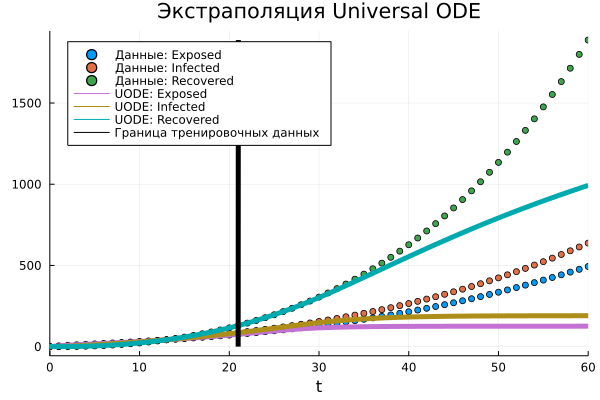
\includegraphics[width=\linewidth]{universalode_extrapolation.png}
							\caption{Экстраполяция обученного UODE.}
							\centering
						\end{minipage}
						\centering
					\end{figure}
				\end{center}
			\end{frame}
			
		\subsection{Модель Лотки-Вольтерра}
			
			\begin{frame}
				\frametitle{Примеры применения UDE} 
				\framesubtitle{Модель Лотки-Вольтерра}
					\begin{itemize}
						\item Модель Лотки-Вольтерра:
						\begin{displaymath}
							\begin{gathered}
							\dot{x} = \alpha x - \beta x y \\
							\dot{y} = -\gamma y + \delta x y
							\end{gathered}
						\end{displaymath}
						\item Забыли о вторых слагаемых в правых частях:
						\begin{displaymath}
						\begin{gathered}
							\dot{x} = \alpha x + U_x(x,y) \\
							\dot{y} = -\gamma y + U_y(x,y)
						\end{gathered}
						\end{displaymath}
						\item Зайцы экспоненциально плодятся в отсутствии хищника
						\item Волки экспоненциально умирают из-за отсутвия добычи
						\item Механизм взаимодействия не знаем =( 
					\end{itemize}
			\end{frame}
		
			\begin{frame}
				\frametitle{Примеры применения UDE} 
				\framesubtitle{Модель Лотки-Вольтерра}
				\begin{center}
					К счастью, у нас в руках оказались данные (Hudson-Bay), которые могут описываться этой моделью.
					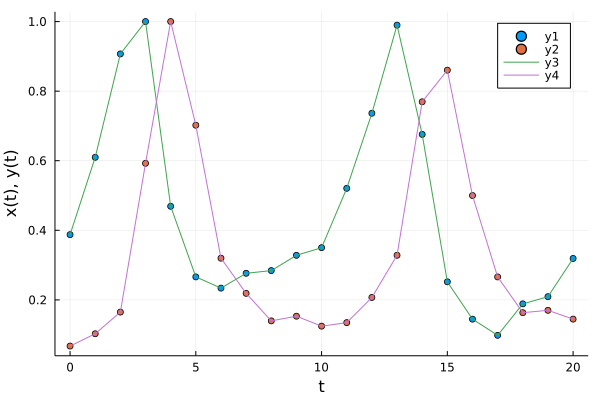
\includegraphics[width=0.7\linewidth]{data.png}
				\end{center}
			\end{frame}
		
			\begin{frame}
				\frametitle{Примеры применения UDE} 
				\framesubtitle{Модель Лотки-Вольтерра}
				\begin{center}
					Использование SINDy просто на исходных данных результата не даёт.
					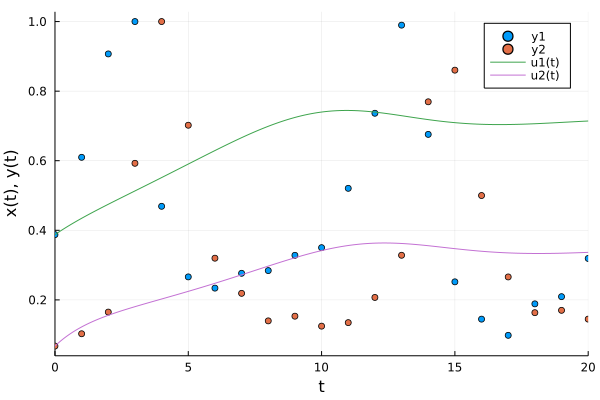
\includegraphics[width=0.7\linewidth]{sindy_solo.png}
				\end{center}
			\end{frame}
	
			\begin{frame}
				\frametitle{Примеры применения UDE} 
				\framesubtitle{Модель Лотки-Вольтерра}
				\begin{center}
					Обучаем наш UODE и смотрим на результат.
					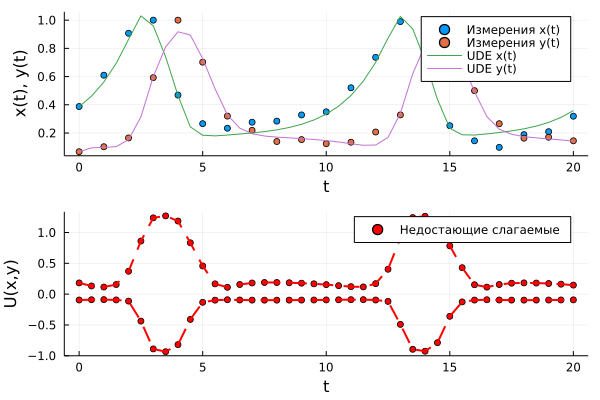
\includegraphics[width=0.8\linewidth]{ude_missing_term_predict_lotka_new.png}
				\end{center}
			\end{frame}
		
			\begin{frame}
				\frametitle{Примеры применения UDE} 
				\framesubtitle{Модель Лотки-Вольтерра}
				\begin{center}
					\begin{itemize}
						\item На полученном результате можем снова попробовать применить SINDy и получаем: \\
						Differential(t)(u[1]) = $p_1$*u[1]*u[2]\\
						Differential(t)(u[2]) = $p_2$*u[1]*u[2]\\
						(-1.56, 2.4)\\
						\item Здесь была использована библиотека полиномов до 3 степени включительно, а также $\sin{u}, \cos{u}$. 
						\item UODE + SINDy восстановили модель Лотки-Вольтерра!
						\item При этом коэффициенты в полученной модели всё ещё можно улучшить, чтобы добиться большей точности
					\end{itemize}
				\end{center}
			\end{frame}
		
			\begin{frame}
				\frametitle{Примеры применения UDE} 
				\framesubtitle{Модель Лотки-Вольтерра}
				\begin{center}
					Обучаем параметры ($\alpha, \beta, \gamma, \delta$) полученной модели под исходные данные. Получили $\alpha \approx 0.557, \beta \approx 0.826, \gamma \approx -1.7, \delta \approx 2.04$.
					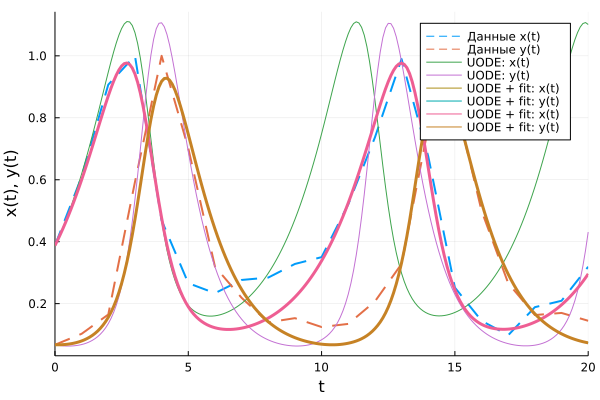
\includegraphics[width=0.7\linewidth]{recover_fit.png}
				\end{center}
			\end{frame}
		
			\begin{frame}
				\frametitle{Примеры применения UDE} 
				\framesubtitle{Модель Лотки-Вольтерра}
				\begin{center}
					Имея хорошую модель, можем экстраполировать её на большие времена!
					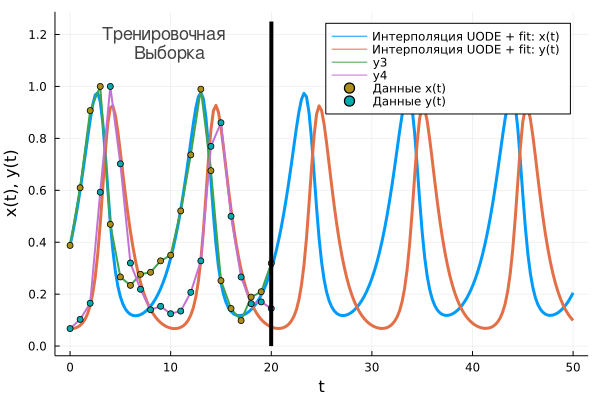
\includegraphics[width=0.7\linewidth]{full_lotka.png}
				\end{center}
			\end{frame}
		
		
	\section*{Литература}
	
		\begin{frame}
			\frametitle{Список литературы} 
				\begin{itemize}
					\item Christopher Rackauckas and Yingbo Ma and Julius Martensen and Collin Warner and Kirill Zubov and Rohit Supekar and Dominic Skinner and Ali Ramadhan and Alan Edelman. Universal Differential Equations for Scientific Machine Learning.
					\item Steven L. Brunton, Joshua L. Proctor, and J. Nathan Kutz. Discovering governing equations from data by sparse identification of nonlinear dynamical systems. 
					\item Maziar Raissi, Paris Perdikaris, and George Em Karniadakis. Physics Informed Deep Learning (Part I): Data-driven Solutions of Nonlinear Partial Differential Equations
					\item Silver, D., Schrittwieser, J., Simonyan, K. et al. Mastering the game of Go without human knowledge. Nature 550, 354–359 (2017). https://doi.org/10.1038/nature24270
				\end{itemize}
			
		\end{frame}

\end{document}